\documentclass[11pt]{article}

\usepackage[T1]{fontenc}
\usepackage[utf8]{inputenc}
\usepackage[margin=1in]{geometry}
\usepackage{amsmath}
\usepackage{amssymb}
\usepackage{booktabs}
\usepackage{tabularx}
\usepackage{array}
\usepackage{xcolor}
\usepackage{listings}
\usepackage{tikz}
\usepackage[hidelinks]{hyperref}

% Inline code shorthand: monospaced, but with line-break opportunities after
% underscores so long identifiers/paths don't overflow the text block.
\newcommand{\code}[1]{\texttt{\def\_{\textunderscore\allowbreak}#1}}

% Let TeX stretch the last line a little rather than overflowing the margin.
\setlength{\emergencystretch}{3em}

\lstset{
  basicstyle=\ttfamily\small,
  breaklines=true,
  frame=single,
  framesep=4pt,
  language=Python,
  keywordstyle=\color{blue!60!black},
  commentstyle=\color{gray},
  stringstyle=\color{green!40!black},
  showstringspaces=false,
  columns=fullflexible,
}

% Plain (non-language) listing style for verbatim program output.
\lstdefinestyle{plain}{language={},keywordstyle=\ttfamily,basicstyle=\ttfamily\footnotesize,breaklines=false}

\title{Propagation of energy units through pymatgen's
\texttt{HeisenbergMapper}}
\author{Luca Frey}
\date{\today}

\begin{document}
\maketitle

\begin{abstract}
\noindent
We trace energy, and its units, through pymatgen's \code{HeisenbergMapper}, from
the input total energies to the serialised \code{HeisenbergModel}. The only
normalisation applied is division by the magnetic-ion count, so the mapper works
internally in eV per magnetic ion and reports couplings in meV per magnetic ion
(despite the ``meV/atom'' label in the source). The fit recovers the physical
exchange constants---up to that ion count---only if every ordering shares one
supercell size. A worked example and a verification test
(Appendices~\ref{app:code}--\ref{app:output}) show that mixing sizes breaks the
fit in two independent ways, and that pymatgen's \code{MagneticStructureEnumerator}
(which drives the \code{MagneticOrderingsMaker} workflow) produces mixed sizes by
construction---so this is the default code path, not an edge case.
\end{abstract}

\section{Introduction}

This note follows the energy, and its units, from the public interface of
\code{HeisenbergMapper} to the \code{HeisenbergModel} it writes out. We assume
the inputs are already available: a list of magnetic structures, each carrying a
\code{magmom} site property, and a list of total energies $E_k^{\mathrm{tot}}$
(eV), each the energy of the whole supercell of ordering $k$. Line references in
Secs.~\ref{sec:ingestion}--\ref{sec:example} are to \code{heisenberg.py}; the
enumerator references in Sec.~\ref{sec:trigger} are to \code{analyzer.py} and to
atomate2.

\section{Notation and energy model}

\begin{table}[h]
\centering
\begin{tabularx}{\textwidth}{@{}l X l@{}}
\toprule
Symbol & Meaning & Unit \\
\midrule
$E_k^{\mathrm{tot}}$ & total DFT energy of ordering $k$ (whole supercell) & eV \\
$N_k^{\mathrm{mag}}$ & number of magnetic ions in ordering $k$ & --- (count) \\
$\varepsilon_k$ & per-mag-ion energy, $E_k^{\mathrm{tot}}/N_k^{\mathrm{mag}}$ & eV / mag ion \\
$s_i$ & local moment (\code{magmom}) on ion $i$, used as a bare number & value in $\mu_B$ \\
$J_{ab}$ & exchange constant for neighbour class $ab$ (nn/nnn/\dots) & see Sec.~\ref{sec:fit} \\
$E_0$ & spin-independent (nonmagnetic) reference energy & eV / mag ion \\
\bottomrule
\end{tabularx}
\end{table}

\noindent
The model is collinear, with moments entering as dimensionless scalars (their
bare $\mu_B$ values), so the energy unit is carried entirely by $J$:
\begin{equation}
E^{\mathrm{tot}} = E_0 - \sum_{\langle i,j\rangle} J_{ij}\, s_i\, s_j ,
\label{eq:model}
\end{equation}
the sum running over unique neighbour bonds $\langle i,j\rangle$.

\section{Ingestion and normalisation}
\label{sec:ingestion}

The constructor routes inputs through \code{HeisenbergScreener.\_do\_cleanup}
(\code{:696}), which (i) restricts each structure to its magnetic sublattice via
\code{get\_structure\_with\_only\_magnetic\_atoms}, so that \code{len(s)} becomes
$N_k^{\mathrm{mag}}$ (\code{:717--722}); (ii) performs the pipeline's single unit
conversion (\code{:725}),
\begin{equation}
  \varepsilon_k = \frac{E_k^{\mathrm{tot}}}{N_k^{\mathrm{mag}}}
  \qquad [\text{eV}] \longrightarrow [\text{eV/mag ion}] ;
\label{eq:norm}
\end{equation}
and (iii) removes degenerate orderings (tolerance $10^{-6}$~eV/mag ion) and sorts
by ascending $\varepsilon_k$ (\code{:732--754}). The result is stored as
\code{self.energies} (\code{:83}); the total energies are not retained. Note that
the divisor is the \emph{magnetic-ion} count, never the total atom count.

\section{The design matrix}
\label{sec:design}

\code{\_get\_exchange\_df} (\code{:229}) builds one row per ordering, with an
\code{E} column (left-hand side), an \code{E0} column, and one column per
neighbour class. For ordering $k$:
\begin{itemize}
  \item \textbf{\code{E}} $=\varepsilon_k$ (\code{:330}), in eV/mag ion;
  \item \textbf{coupling column} $C_{ab,k}$: the code accumulates $-s_i s_j$ over
        every ion $i$ and neighbour $j$ (\code{:318--321}); each bond is counted
        from both endpoints, and the factor $\tfrac12$ at \code{:338} removes the
        double count, leaving
        \begin{equation}
          C_{ab,k} = -\!\!\sum_{\langle i,j\rangle\,\in\,ab\ \text{in cell }k}\!\! s_i\, s_j
          \qquad(\text{a pure number, summed over \emph{all} bonds in the cell});
          \label{eq:coeff}
        \end{equation}
  \item \textbf{\code{E0}} $=1$ (\code{:339}), a dimensionless constant column.
\end{itemize}
Each row is therefore
\begin{equation}
  \varepsilon_k = E_0\cdot 1 + \sum_{ab} J_{ab}\, C_{ab,k} .
  \label{eq:row}
\end{equation}
With $\varepsilon_k$ in eV/mag ion and $C_{ab,k}$ a pure number, dimensional
balance fixes $[E_0]=[J_{ab}]=\text{eV/mag ion}$. The matrix is then made square
(\code{:342--349}): all-zero columns dropped, rows truncated to match the number
of unknowns.\footnote{The all-zero-column guard (\code{:341--345}) is buggy and
pandas-version dependent, but fires only in the degenerate case where some class
has $\sum s_i s_j=0$ in \emph{every} ordering; ordinary multi-$J$ fits never reach
it.}

\section{Solving the system}
\label{sec:fit}

\code{get\_exchange} (\code{:353}) solves $H\,x=\boldsymbol\varepsilon$ for
$x=(E_0,J_{\mathrm{nn}},J_{\mathrm{nnn}},\dots)^{\mathsf T}$, where $H$ collects
the \code{E0} and coupling columns and
$\boldsymbol\varepsilon=(\varepsilon_1,\dots,\varepsilon_n)^{\mathsf T}$. It
inverts directly (\code{:376--378}), so the raw solution is in eV/mag ion; then
$J$ (but not $E_0$) is scaled to meV (\code{:381}):
\begin{equation}
  x = H^{-1}\boldsymbol\varepsilon \ [\text{eV/mag ion}],
  \qquad
  J_{ab}\mathrel{*}{=}1000 \ \Rightarrow\ J_{ab}\ [\text{meV/mag ion}]
  \quad(\text{source label: ``meV/atom''}).
\end{equation}
If fewer than three independent classes exist, the matrix route is bypassed
(\code{:367--373}) and a single average $\langle J\rangle =
(\varepsilon_{\mathrm{afm}}-\varepsilon_{\mathrm{fm}})/\langle|s|\rangle^2$ (then
$\times10^3$) is returned (\code{estimate\_exchange}, \code{:454--487}), likewise
in meV/mag ion.

\section{What is written out, and the unit trace}
\label{sec:summary}

The serialised \code{HeisenbergModel} (\code{:624}) stores: \code{energies}
$=\varepsilon_k$ (eV/mag ion); \code{ex\_mat} (\code{E} column eV/mag ion,
coupling columns pure numbers); \code{ex\_params} and \code{javg} (meV/mag ion);
and \code{igraph} edge weights (meV/mag ion, labelled \code{"meV"}). The energy
unit changes exactly twice along the pipeline, summarised in
Table~\ref{tab:units}.

\begin{table}[h]
\centering
\begin{tabularx}{\textwidth}{@{}l X l@{}}
\toprule
Stage & Operation (source) & Unit \\
\midrule
Input        & $E_k^{\mathrm{tot}}$, whole supercell                                 & eV \\
Normalise    & $\varepsilon_k=E_k^{\mathrm{tot}}/N_k^{\mathrm{mag}}$ (Eq.~\ref{eq:norm}, \code{:725}) & eV / mag ion \\
Design+solve & $H\,x=\boldsymbol\varepsilon$ for $E_0,\{J_{ab}\}$ (Secs.~\ref{sec:design}--\ref{sec:fit}) & eV / mag ion \\
meV scale    & $J_{ab}\mathrel{*}{=}1000$; $E_0$ left in eV (\code{:381})            & meV / mag ion \\
\midrule
Output $J$   & \code{ex\_params}, \code{javg}                                        & meV / mag ion \\
Output $E$   & \code{model.energies} $=\varepsilon_k$                                & eV / mag ion \\
\bottomrule
\end{tabularx}
\caption{Energy unit in force at each stage. The total atom count never enters.}
\label{tab:units}
\end{table}

\section{Consistency condition on supercell size}
\label{sec:consistency}

Write the supercell of ordering $k$ as $n_k$ primitive cells, with $\nu$ magnetic
ions per primitive cell. Because the ordering is periodic with that cell, the
ion count, the bond sum~\eqref{eq:coeff}, and the nonmagnetic energy are all
proportional to $n_k$:
\begin{equation}
  N_k^{\mathrm{mag}} = \nu\, n_k,
  \qquad
  C_{ab,k} = n_k\, c_{ab,k},
  \qquad
  E_{0,k}^{\mathrm{tot}} = n_k\, e_0,
  \label{eq:scaling}
\end{equation}
where $c_{ab,k}$ and $e_0$ are the per-primitive-cell (intensive) quantities.
The physical total energy $E_k^{\mathrm{tot}} = n_k e_0 + \sum_{ab}
J_{ab}^{\mathrm{phys}} C_{ab,k}$, divided by $N_k^{\mathrm{mag}}$
(Eq.~\ref{eq:norm}), gives the left-hand side the code actually fits:
\begin{equation}
  \varepsilon_k
  = \frac{e_0}{\nu} + \sum_{ab}\frac{J_{ab}^{\mathrm{phys}}}{\nu}\,c_{ab,k}
  \qquad(\text{intensive: independent of } n_k).
  \label{eq:eps_intensive}
\end{equation}
Equating this with the design row~\eqref{eq:row}, and using
$C_{ab,k}=n_k c_{ab,k}$,
\begin{equation}
  \varepsilon_k
  = E_0\cdot\underbrace{1}_{\text{column}}
  + \sum_{ab} J_{ab}\,\underbrace{n_k\, c_{ab,k}}_{C_{ab,k}} .
  \label{eq:row_scaled}
\end{equation}
The asymmetry is now explicit. The left-hand side is intensive and the \code{E0}
column is unity, so a \emph{single} $E_0=e_0/\nu$ satisfies every row whatever the
supercell size. But the coupling columns carry $C_{ab,k}=n_k c_{ab,k}\propto n_k$,
so they are effectively extensive: matching~\eqref{eq:eps_intensive}
and~\eqref{eq:row_scaled} forces
\begin{equation}
  J_{ab} = \frac{J_{ab}^{\mathrm{phys}}}{N_k^{\mathrm{mag}}},
\end{equation}
which is one value across all rows only if $N_k^{\mathrm{mag}}$ (equivalently
$n_k$) is the \emph{same} for every ordering. Then the couplings come out as
$J^{\mathrm{phys}}/N^{\mathrm{mag}}$ (the ``per magnetic ion'' of the reported
units). When the sizes differ, no single $J$ set fits, and two separate things go
wrong; the worked example (Sec.~\ref{sec:example}) exhibits both.

\section{Worked example and verification}
\label{sec:example}

We take the smallest system with two neighbour classes: the $J_1$--$J_2$ square
lattice of one magnetic species ($\nu=1$, $|s_i|=1$), with the three orderings of
Fig.~\ref{fig:orderings}---ferromagnet (FM), row-stripe AFM (Stripe), and
checkerboard N\'eel---and the Hamiltonian~\eqref{eq:model} with
$J_{\mathrm{nn}}^{\mathrm{phys}}=+12$~meV, $J_{\mathrm{nnn}}^{\mathrm{phys}}=-4$~meV,
$e_0=-5$~eV. These are exactly the parameters of the verification test in
Appendix~\ref{app:code}, whose verbatim output is Appendix~\ref{app:output}; the
matrices below are that output, annotated. Since $\varepsilon_k$ is intensive
(Eq.~\ref{eq:eps_intensive}), the $\varepsilon$ column is the same in every
matrix; only $C_{ab,k}$ changes with cell size.

\begin{figure}[h]
\centering
\begin{minipage}[t]{0.31\textwidth}\centering
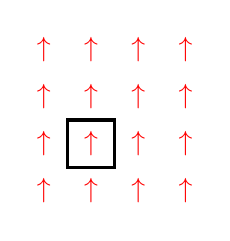
\begin{tikzpicture}[scale=0.6]
  \foreach \x in {0,1,2,3}{\foreach \y in {0,1,2,3}{\node[red] at (\x,\y){$\uparrow$};}}
  \draw[very thick] (0.5,0.5) rectangle (1.5,1.5);
\end{tikzpicture}\\[3pt]
{\footnotesize (a) FM --- cell $1\times1$, $N=1$}
\end{minipage}
\hfill
\begin{minipage}[t]{0.31\textwidth}\centering
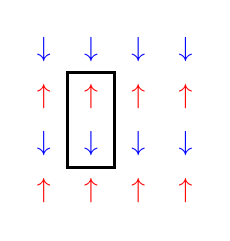
\begin{tikzpicture}[scale=0.6]
  \foreach \x in {0,1,2,3}{\foreach \y in {0,2}{\node[red]  at (\x,\y){$\uparrow$};}}
  \foreach \x in {0,1,2,3}{\foreach \y in {1,3}{\node[blue] at (\x,\y){$\downarrow$};}}
  \draw[very thick] (0.5,0.5) rectangle (1.5,2.5);
\end{tikzpicture}\\[3pt]
{\footnotesize (b) Stripe --- cell $1\times2$, $N=2$}
\end{minipage}
\hfill
\begin{minipage}[t]{0.31\textwidth}\centering
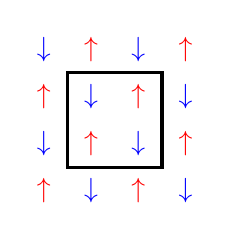
\begin{tikzpicture}[scale=0.6]
  \foreach \x in {0,1,2,3}{\foreach \y in {0,1,2,3}{
    \pgfmathtruncatemacro{\s}{mod(\x+\y,2)}
    \ifnum\s=0 \node[red] at (\x,\y){$\uparrow$};\else\node[blue] at (\x,\y){$\downarrow$};\fi}}
  \draw[very thick] (0.5,0.5) rectangle (2.5,2.5);
\end{tikzpicture}\\[3pt]
{\footnotesize (c) N\'eel --- cell $2\times2$, $N=4$}
\end{minipage}
\caption{The three orderings. Red $\uparrow$ / blue $\downarrow$ are the collinear
spin directions; nn bonds lie along the axes, nnn along the diagonals. The heavy
box is the minimal magnetic cell ($N=1,2,4$).}
\label{fig:orderings}
\end{figure}

\paragraph{(i) Correct: a common supercell.}
With every ordering in the same $2\times2$ cell ($N=4$ throughout):
\begin{equation*}
\begin{array}{l|c|ccc|c}
\text{ordering} & N_k & E_0 & C_{\mathrm{nn}} & C_{\mathrm{nnn}} & \varepsilon~[\mathrm{eV/ion}]\\\hline
\text{FM}     & 4 & 1 & -8 & -8 & -5.016\\
\text{Stripe} & 4 & 1 &  0 & +8 & -5.008\\
\text{N\'eel} & 4 & 1 & +8 & -8 & -4.968
\end{array}
\end{equation*}
The solve returns $E_0=-5.0$~eV, $J_{\mathrm{nn}}=+3.0$, $J_{\mathrm{nnn}}=-1.0$~meV,
i.e.\ exactly $J^{\mathrm{phys}}/4$ and $e_0$ (Appendix~\ref{app:output}, ``common
$2\times2$''; the test asserts this). Every row carries the same factor $N=4$,
which cancels in the solve.

\paragraph{(ii) Failure mode 1 --- the normalisation asymmetry.}
Put each ordering in its minimal cell, but suppose $C_{ab,k}$ were still computed
faithfully. By Eq.~\eqref{eq:scaling} the rows then scale by their own $n_k=N_k$
(FM by $\tfrac14$, Stripe by $\tfrac12$ relative to the common cell), while
$\varepsilon$ is unchanged:
\begin{equation*}
\begin{array}{l|c|ccc|c}
\text{ordering} & N_k & E_0 & C_{\mathrm{nn}} & C_{\mathrm{nnn}} & \varepsilon~[\mathrm{eV/ion}]\\\hline
\text{FM}     & 1 & 1 & -2 & -2 & -5.016\\
\text{Stripe} & 2 & 1 &  0 & +4 & -5.008\\
\text{N\'eel} & 4 & 1 & +8 & -8 & -4.968
\end{array}
\end{equation*}
No single $(E_0,\{J_{ab}\})$ can satisfy rows demanding $J^{\mathrm{phys}}/1$,
$/2$, $/4$ at once; the (non-singular) solve returns the meaningless
$E_0\approx-5.01$~eV, $J_{\mathrm{nn}}\approx+4.67$, $J_{\mathrm{nnn}}\approx-0.22$~meV.
This is exactly Eq.~\eqref{eq:row_scaled} with non-constant $n_k$.

\paragraph{(iii) Failure mode 2 --- the unique-site map.}
The code never even reaches matrix (ii), because the column scheme
(\code{unique\_site\_ids}) is built once from \code{ordered\_structures[0]}
(\code{:91}), assuming all orderings share one site indexing. After the energy
sort the lowest-energy ordering is first---here FM in its $1\times1$ cell---so
$\code{unique\_site\_ids}=\{(0,)\!:0\}$ knows only index $0$. Site indices $\ge1$
are mapped to \code{None} (\code{:285--305}) and their bonds are silently dropped
(\code{:318--321}). The surviving matrix is
\begin{equation*}
\begin{array}{l|c|ccc|c}
\text{ordering} & N_k & E_0 & C_{\mathrm{nn}} & C_{\mathrm{nnn}} & \varepsilon~[\mathrm{eV/ion}]\\\hline
\text{FM}     & 1 & 1 & -2 & -2 & -5.016\\
\text{Stripe} & 2 & 1 & -1 &  0 & -5.008\\
\text{N\'eel} & 4 & 1 &  0 &  0 & -4.968
\end{array}
\end{equation*}
(N\'eel loses all bonds; Stripe keeps only its $0$--$0$ image nn). The solve
returns $E_0=-4.97$~eV, $J_{\mathrm{nn}}=+40$, $J_{\mathrm{nnn}}=-16$~meV---pure
nonsense, with no error raised (Appendix~\ref{app:output}, ``mixed minimal
cells''). Table~\ref{tab:threecases} collects the three outcomes.

\begin{table}[h]
\centering
\begin{tabularx}{\textwidth}{@{}X c c c@{}}
\toprule
Scenario & $E_0$ & $J_{\mathrm{nn}}$ [meV] & $J_{\mathrm{nnn}}$ [meV] \\
\midrule
(i) Common $2\times2$ cell (correct)        & $-5.0$~eV  & $+3.0$  & $-1.0$  \\
(ii) Mixed cells, faithful coeff.\ (hypothetical) & $-5.01$~eV & $+4.67$ & $-0.22$ \\
(iii) Mixed cells, actual code              & $-4.97$~eV & $+40$   & $-16$   \\
\bottomrule
\end{tabularx}
\caption{Couplings in the three scenarios. Physical truth: $J_{\mathrm{nn}}=+12$,
$J_{\mathrm{nnn}}=-4$~meV; only (i) recovers it (as $J^{\mathrm{phys}}/N$).}
\label{tab:threecases}
\end{table}

\subsection{When is the bad case hit? It is the main code path}
\label{sec:trigger}

The fit is only wrong when the orderings handed to it differ in
$N_k^{\mathrm{mag}}$. That is precisely what pymatgen's
\code{MagneticStructureEnumerator} (the engine behind atomate2's
\code{MagneticOrderingsMaker}) produces. The ferromagnetic ordering is kept at
the \emph{primitive} cell size, whereas the antiferromagnetic and ferrimagnetic
strategies are enumerated over supercells up to
\begin{equation}
  \texttt{max\_cell\_size} = \max\!\big(1,\ \lfloor 4/N_{\mathrm{mag,prim}}\rfloor\big)
  \qquad(\code{analyzer.py:802}),
\end{equation}
so for a primitive cell with a single magnetic site this enumerates orderings in
cells of $1$, $2$, $3$, and $4$ formula units at once. Running the enumerator on
a one-site cell indeed returns orderings with
$N_k^{\mathrm{mag}}\in\{1,2,4\}$. The atomate2 exchange flow
(\code{ExchangeMaker.make\_from\_ordering\_doc}) then feeds \emph{all} of these to
\code{HeisenbergMapper}, sorted by energy but with no size filtering. Mixed
supercell sizes are therefore the normal output of the standard workflow, and
both failure modes above lie on the main code path---not on an edge case. A
correct fit requires restricting the inputs to a single common
$N_k^{\mathrm{mag}}$ (or dividing the coupling columns by $N_k^{\mathrm{mag}}$ as
well, which would make Eq.~\eqref{eq:row_scaled} fully intensive).

\section{Conclusion}

\code{HeisenbergMapper} applies one normalisation---division by the magnetic-ion
count---so it works in eV/mag ion and reports couplings in meV/mag ion, despite
the ``meV/atom'' label. The fit equals $J^{\mathrm{phys}}/N^{\mathrm{mag}}$ only
when all orderings share one supercell size. The left-hand side is intensive (so
one $E_0$ fits any size), but the coupling columns scale as $C_{ab,k}=n_k
c_{ab,k}$ and are effectively extensive, so unequal sizes are ill-posed (failure
mode~1); separately, \code{unique\_site\_ids} is built from
\code{ordered\_structures[0]} alone and silently drops bonds for larger cells
(failure mode~2). Since \code{MagneticStructureEnumerator} generates mixed sizes
by design (Sec.~\ref{sec:trigger}), these are the default behaviour, not edge
cases.

\appendix

\section{Verification test \texttt{test\_heisenberg\_fit.py}}
\label{app:code}

The test builds the three orderings, assigns each a total energy from
Eq.~\eqref{eq:model} computed analytically on the lattice (independent of
pymatgen's neighbour enumeration), and asserts that the common-cell fit recovers
$J^{\mathrm{phys}}/N$ and $E_0=e_0$; the mixed-cell block is a (non-asserted)
demonstration of Sec.~\ref{sec:example}(iii).

\lstinputlisting[language=Python]{test_heisenberg_fit.py}

\section{Test output}
\label{app:output}

\begin{lstlisting}[style=plain]
physical truth: e0 = -5.000 eV, Jnn = +12.0 meV, Jnnn = -4.0 meV

=== common 2x2 supercell (N = 4 for all orderings) ===
  FM      cell=(2, 2) N=4  E_tot=-20.064000 eV
  Stripe  cell=(2, 2) N=4  E_tot=-20.032000 eV
  Neel    cell=(2, 2) N=4  E_tot=-19.872000 eV
  unique_site_ids: {(0, 1, 2, 3): 0}
  ex_mat:
           E  E0  0-0-nn  0-0-nnn
    0 -5.016   1    -8.0     -8.0
    1 -5.008   1     0.0      8.0
    2 -4.968   1     8.0     -8.0
  fitted : {'nn': 3.0, 'nnn': -1.0, 'E0': -5.0}
  expect : {'nn': 3.0, 'nnn': -1.0, 'E0': -5.0}   (Jnn,Jnnn = J_phys/N)
  -> PASS

=== mixed minimal cells: FM 1x1, Stripe 1x2, Neel 2x2 ===
  FM      cell=(1, 1) N=1  E_tot=-5.016000 eV
  Stripe  cell=(1, 2) N=2  E_tot=-10.016000 eV
  Neel    cell=(2, 2) N=4  E_tot=-19.872000 eV
  unique_site_ids: {(0,): 0}
  ex_mat:
           E  E0  0-0-nn  0-0-nnn
    0 -5.016   1    -2.0     -2.0
    1 -5.008   1    -1.0      0.0
    2 -4.968   1     0.0      0.0
  fitted : {'E0': -4.968, '0-0-nn': 40.0, '0-0-nnn': -16.0}
  NOTE: not expected to match J_phys/N -- mixing supercell sizes
        breaks the fit (heisenberg_energy_units.tex, Sec. 8):
        unique_site_ids is built only from the first structure, so
        bonds touching higher site indices are silently dropped.
\end{lstlisting}

\end{document}
